\section{Modelo de Banco de Dados}
Para o desenvolvimento da aplicação foram elaborados previamente modelos de representação do banco de dados. Tais modelos auxiliam a ter uma visão da aplicação antes que seja de fato desenvolvida.
\subsection{Modelo Entidade Relacionamento - MER}
O \gls{mer} explica muito sobre a aplicação e já aponta algumas regras de negócio.
Nele foram definidas as seguintes entidades e relacionamentos:
\begin{itemize}
	\item \emph{CUSTOMER}: Entidade que representa um cliente.
	\begin{itemize}
		\item \textbf{\textit{refers:}} um cliente (\emph{CUSTOMER}) pode ou não indicar (\textit{refers}) outros clientes e um cliente é indicado por nenhum ou um único cliente.
		\item \textbf{\textit{makes:}} um cliente faz (\emph{makes}) ou não agendamentos (\emph{APPOINTMENT}).
	\end{itemize}
	\item \emph{APPOINTMENT}: Entidade que representa um agendamento.
	\begin{itemize}
		\item \textbf{\textit{makes}}: um agendamento (\emph{APPOINTMENT}) é feito (\textit{makes}) por um cliente (\emph{CUSTOMER}). 
		\item \textbf{\textit{has}}: um agendamento (\emph{APPOINTMENT}) tem (\textit{has}) ou não uma avaliação (\emph{RATING}).
		\item \textbf{\textit{sends}}: um agendamento (\emph{APPOINTMENT}) envia (\textit{sends}) ao menos uma notificação (\emph{NOTIFICATION}).
		\item \textbf{\textit{includes}}: um agendamento (\emph{APPOINTMENT}) inclui (\textit{includes}) uma oferta (\emph{OFFER}).
	\end{itemize}
	\item \emph{RATING}: Entidade que representa a avaliação de um agendamento.
	\begin{itemize}
		\item \textbf{\textit{has:}} uma avaliação (\emph{RATING}) é tida (\textit{has}) por um agendamento (\emph{APPOINTMENT}).
	\end{itemize}
	\item \emph{NOTIFICATION}: Entidade que representa uma notificação.
	\begin{itemize}
		\item \textbf{\textit{sends:}} uma notificação (\emph{NOTIFICATION}) é enviada por (\textit{sends}) um agendamento (\emph{APPOINTMENT}).
	\end{itemize}
	\item \emph{OFFER}: Entidade associativa que representa a oferta (\textit{offers}) de um serviço (\emph{SERVICE}) por um funcionário (\emph{EMPLOYEE}).
	\begin{itemize}
		\item \textbf{\textit{includes}}: uma oferta (\emph{OFFER}) pode ou não ser incluida (\textit{includes}) em muitos agendamentos (\emph{APPOINTMENT}). 
	\end{itemize}
	\item \emph{EMPLOYEE}: Entidade que representa um funcionário.
	\begin{itemize}
		\item \textbf{\textit{offers}}: um funcionário (\emph{EMPLOYEE}) oferece (\textit{offers}) ou não muitos serviços (\emph{SERVICE}).
		\item \textbf{\textit{has}}: um funcionário (\emph{EMPLOYEE}) tem (\textit{has}) ou não muitos turnos (\emph{SHIFT}).
		\item \textbf{\textit{has}}: um funcionário (\emph{EMPLOYEE}) tem (\textit{has}) ao menos um papel (\emph{ROLE}).
	\end{itemize}
	\item \emph{SERVICE}: Entidade que representa um serviço no salão de beleza.
	\begin{itemize}
		\item \textbf{\textit{offers}}: um serviço (\emph{SERVICE}) é oferecido (\textit{offers}) ou não por muitos funcionários (\emph{EMPLOYEE}).
	\end{itemize}
	\item \emph{SHIFT}: Entidade que representa os turnos de trabalho de um funcionário.
	\begin{itemize}
		\item \textbf{\textit{has}}: um turno (\emph{SHIFT}) é tido (\textit{has}) por um funcionário (\emph{EMPLOYEE}).
	\end{itemize}
	\item \emph{ROLE}: Entidade que representa os papéis que um funcionário possui na plataforma.
	\begin{itemize}
		\item \textbf{\textit{has}}: um papel (\emph{ROLE}) é tido ou não (\textit{has}) por muitos funcionários (\emph{EMPLOYEE}).
		\item \textbf{\textit{has}}: um papel (\emph{ROLE}) tem (\textit{has}) ao menos uma permissão (\emph{PERMISSIONS}).
	\end{itemize}
	\item \emph{EMPLOYE\_ROLE}: Entidade associativa auxiliar para \emph{EMPLOYEE} e \emph{ROLE}.
	\item \emph{PERMISSIONS}: Entidade que representa as permissões que cada papel provê.
	\begin{itemize}
		\item \textbf{\textit{has}}: uma permissão (\emph{PERMISSIONS}) é tida (\textit{has}) ou não por muitos papeis (\emph{ROLE}).
\end{itemize}
	\item \emph{ROLE\_PERMISSION}: Entidade associativa auxiliar para \emph{ROLE} e \emph{PERMISSIONS}.
\end{itemize}
\begin{figure}[h!tbp]
	\centering
	\caption{MER}
	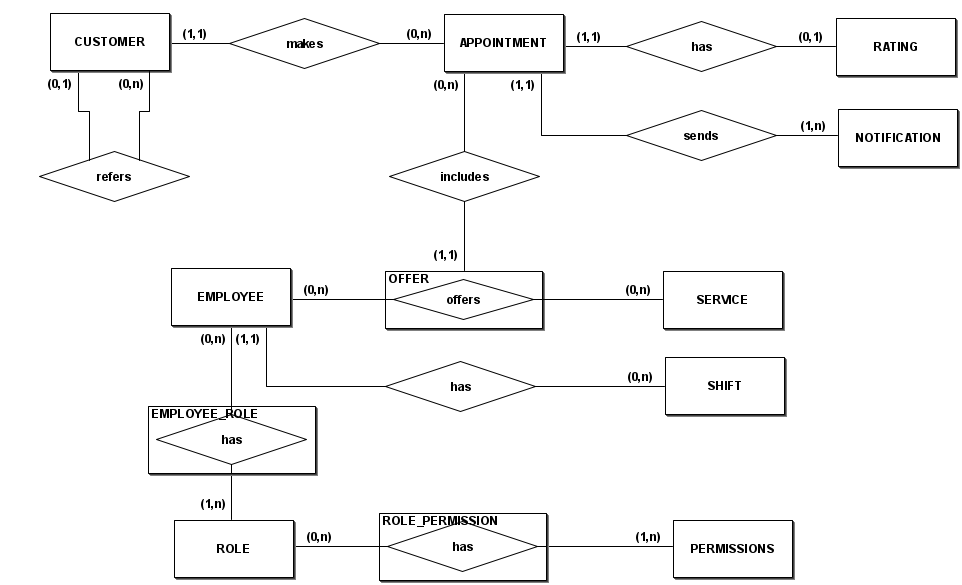
\includegraphics[width=1\textwidth]{cap04-desenvolvimento/images/4-7-1-modelo-entidade-relacionamento.png}
	\fonte{Produzido pelos autores}
	\label{fig:mer}
\end{figure}
\subsection{Diagrama Entidade Relacionamento - DER}
Após a elaboração do \gls{mer} conforme o entendimento dos requisitos e necessidades da entidade parceira, foi produzido um \gls{der}, a partir do \gls{mer}, que contém a listagem de todos os atributos das entidades modeladas, apresentando seus nomes, o tipo de dado e sua possível categorização como chave primária (identificadora) ou estrangeira.
\begin{figure}[h!tbp]
	\centering
	\caption{DER}
	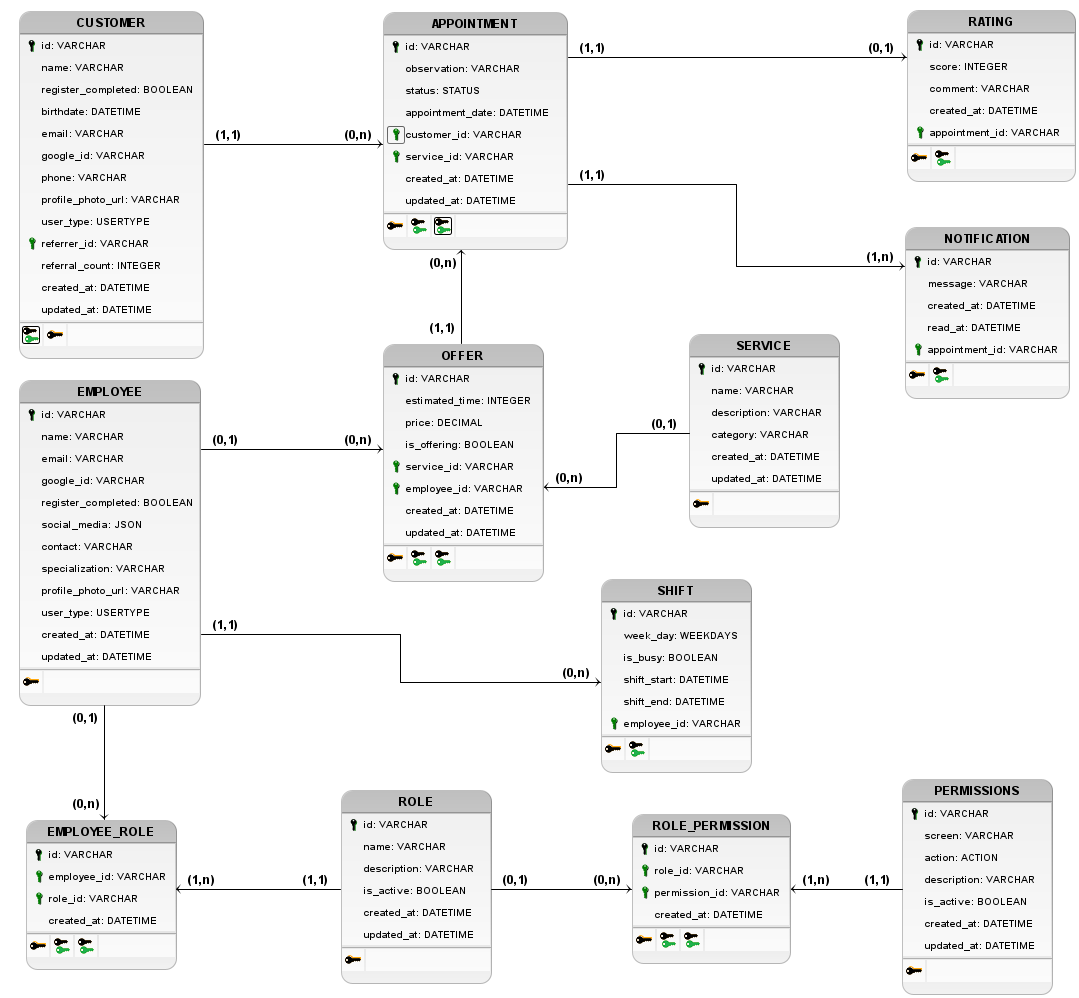
\includegraphics[width=1\textwidth]{cap04-desenvolvimento/images/4-7-2-diagrama-entidade-relacionamento.png}
	\fonte{Produzido pelos autores}
	\label{fig:der}
\end{figure}
\subsection{Dicionário de Dados}
Pensando no modelo físico de banco de dados, também foi elaborado um dicionário de dados referente ao sistema que se enquadra como uma poderosa ferramenta de documentação. Com esse instrumento, qualquer pessoa pode entender como foi pensado os atributos do sistema, como são armazenados e qual seria a finalidade de cada um.
O dicionário descreve:
\begin{itemize}
	\item \textbf{\gls{pk}/\gls{fk}:} Se um atributo é chave primária ou estrangeira.
	\item \textbf{Nome do Campo:} Qual o nome do atributo.
	\item \textbf{Tipo:} Qual o tipo de dado do atributo, como \textit{INT} para valores numéricos inteiros.
	\item \textbf{Descrição:} A descrição do atributo, explicando o que representa na prática.
	\item \textbf{\textit{Null:}} Se o campo pode ser nulo, ou seja, não ter valor atribuído.
	\item \textbf{Tamanho:} O tamanho do atributo, como quantidade de caracteres (\textit{bytes}).
	\item \textbf{Valores permitidos:} Quais os valores permitidos para atributos. Alguns campos utilizam enumerações, por exemplo, que possuem valores definidos previamente.
	\item \textbf{Observações:} Algumas especificidades, como valores padrão, ou de onde uma \gls{fk} foi tomada.
\end{itemize}
Abaixo se encontra um \textit{QR Code} que leva à planilha onde foi elaborado o dicionário de dados desta aplicação.
\begin{figure}[h]
	\centering
	\caption{\emph{QR Code} do Dicionário de Dados}
	\label{fig:qrcode-dicionario-de-dados}
	\scalebox{1.5}{\qrcode{https://docs.google.com/spreadsheets/d/17kJ2aQqjXM-HIXZLWUs257oe_hur0jlTakR0s9KdBrE}}
	\fonte{Produzido pelos autores}
\end{figure}





